\documentclass[12pt]{amsart}
\usepackage{geometry} % see geometry.pdf on how to lay out the page. There's lots.
\usepackage{graphicx}	% Including figure files
\usepackage{amsmath}	% Advanced maths commands
\usepackage{amssymb}	% Extra maths symbols
\usepackage{hyperref}
\usepackage{float}
\floatplacement{figure}{H}
\floatplacement{table}{H} 
\geometry{a4paper} % or letter or a5paper or ... etc

\title{CSE 546: Machine Learning Homework 3}
\author{David P. Fleming}
\date{November 21st, 2016}

%%% BEGIN DOCUMENT
\begin{document}

\maketitle
\tableofcontents

\section*{Introduction}

Please note that a copy of all the code I wrote to answer the questions in this assignment are included in my submission but also located online at \url{https://github.com/dflemin3/CSE_546/tree/master/HW3}.  Some scripts require data, such as MNIST data, to run to completion and were not included on my github due to file size constraints.  The MNIST data is included in the {\tt Data} directory as python {\tt .pkl} files as this compressed format gave me quicker load times for my scripts.

Overall, my code is structured as follows:  There are three main directories included in my submission: {\tt DML}, {\tt Data} and {\tt HW3}. {\tt HW3} contains all the scripts used to run my analysis.  For example to reproduce the answer for Question 1.2, one would run {\tt python hw3$\_1.2.py$}.  All scripts have relative file paths so the code should run and have detailed comments to describe functionality.  In addition, the scripts have flags near the top to control functionality.  By default, I set all flags to true so the script performs the entire analysis and plotting.  The {\tt Data} directory contains both the MNIST dataset. The grader should be able to run my homework scripts without altering this directory.  

The {\tt DML} directory contains all the auxiliary files used to do the computations in the homework scripts and has a logical hierarchy.  For example, the directory {\tt optimization} contains the file {\tt gradient$\_$descent.py} while contains both my batch gradient descent and stochastic gradient descent implementations.  The directory {\tt data$\_$processing} contains the script {\tt mnist$\_$utils.py} which contains my functions used to load and work with the MNIST data.  The directory {\tt classification} contains the file {\tt classifier$\_$utils.py} which contains all things related to binary and softmax classification including the gradients for each respective method for use with a gradient descent algorithm.  The {\tt validation} subdirectory contains {\tt validation.py}.  This file contains all my loss functions such as 0/1 loss and also my implementations for regularization paths for both linear regression and logistic and softmax classification using gradient descent.  Finally, the {\tt regression} directory contains all utilities for a normal or multi-class regression.  In particular, this directory contains the file where my ridge regression implementation lives, {\tt ridge$\_$utils.py}. 

In each section, I try to be explicit with what files I used to perform the computation including the path from the {\tt DML} directory for ease of grading.

%%% QUESTION 0  %%%
\section*{Question 0: Collaborators}
I collaborated with Matt Wilde, Serena Liu, and Janet Matsen for various questions on this assignment.

%%% QUESTION 1 %%%

\section*{Question 1: PCA and reconstruction}

In this question, I derive matrix algebra relations and I use my PCA implementation to reduce the dimensionality of the MNIST dataset and visualize the results.  The code used to solve this question is in the following attached files: {\tt hw3$\_$1.2.py, hw3$\_$1.3.py, hw3$\_$1.4.py} in the {\tt HW3} directory and {\tt classification/classifier$\_$utils.py, regression/regression$\_$utils.py, validation/validation.py, data$\_$processing/mnist$\_$utils.py} in the {\tt DML} directory.

\subsection*{1.0: Details of my PCA implementation}

My PCA implementation performs a SVD on the MNIST training datat $X$ to derive the principal components and the eigenvectors of the empirical covariance matrix, Eqn.~\ref{eqn:sigma}.   Performing PCA using a SVD gives me the following matrices: $u$, $s$, and $v$ where the columns of $v$ are the eigenvectors of Eqn.~\ref{eqn:sigma}.  The eigenvalues of Eqn.~\ref{eqn:sigma} are given by the square of the singular values divided by the length of the dataset, $\lambda = s^2/N$.

To transform the dataset to a lower dimensional space using the first $l$ principal components, the first $l$ columns of $v$, I evaluate
\begin{equation} \label{eqn:pca_transform}
X_{trans} = Xv
\end{equation}
since $X$ is $N \times d$ and the truncated $v$ is $d \times l$ resulting in a lower-dimensional $N \times l$ $X_{trans}$.  I reproject my lower-dimensional transformed data back into``physical'' space via
\begin{equation} \label{eqn:pca_inverse_transform}
X_{approx} = X_{trans}v^T
\end{equation} 
since $X_{trans}$ is $N \times l$ and $v^T$ is $l \times d$ resulting in a $N \times d$ matrix.  Note that $X_{approx} \neq X$ for $l < d$ principal components since using less than the total feature number of principal components instead yields an approximation of the original data when projected back into the original space.

Note that for all questions, I first centered the training data before running PCA.  Specifically, for each feature (column) of $X$, I subtracted off its mean.  In addition to the textbook suggesting this as a good practice, I found that it yielded better performance and hence do so for all PCA questions in this homework set in less explicitly stated otherwise.

\subsection*{1.1: Matrix Algebra Review}

\begin{equation} \label{eqn:sigma}
\Sigma = \frac{1}{N}\sum_i x_i x_i^T
\end{equation}

TODO

\subsection*{1.2: PCA}

Here I performed PCA on the MNIST training data and retained the first 50 principal components and singular values.  The code used to answer this question is located in files: {\tt hw3$\_$1.2.py} in the {\tt HW3} directory and {\tt pca/pca.py} in the {\tt DML} directory.

\subsubsection*{1.2.1}

The eigenvalues $\lambda_1, \lambda_2, \lambda_{10}, \lambda_{30}, \lambda_{50}$ are 332719.1, 243279.9, 80808.5, 23685.7, and 11035.3, respectively. The sum of all eigenvalues is 3428445.4.  Again, I calculate $\lambda = s^2/N$ for singular value $s$ and dataset size $N$.

\subsubsection*{1.2.2}

I plot the fractional reconstruction error for $k \in [1,50]$ for the $k$ principal components in Fig.~\ref{fig:frac_rec_error}.  The fractional reconstruction error is defined as
\begin{equation} \label{eqn:frac_rec_error}
F = 1 - \frac{\sum_{i=1}^k \lambda_i}{\sum_{i=1}^d \lambda_i}
\end{equation}
for $d$ total features and $k$ principal components.  Note how the first principal component is the largest eigenvalue as shown above.
 
\begin{figure}[H]
	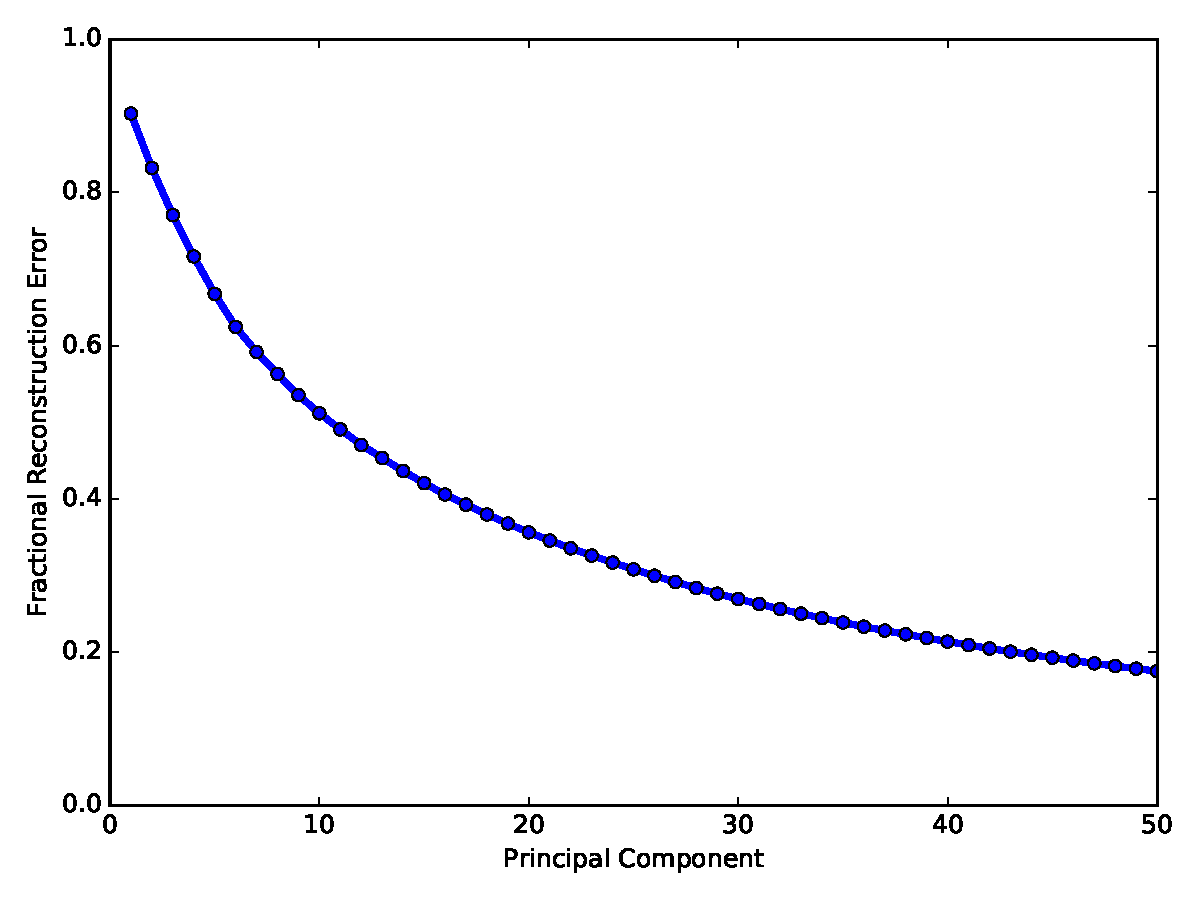
\includegraphics[width=\columnwidth]{fractional_rec_error.pdf}
    \caption{Fractional reconstruction error as a function of $k$ principal components out of $d$ total dimensions for $k \in [1,50]$.}
    \label{fig:frac_rec_error}
\end{figure}


\subsubsection*{1.2.3}

The first eigenvalue, and its corresponding principal component, represent the component of the data that captures the most variance.  That is, the first eigenvalue represents the intensity dimensions.  If the data is not centered, the first eigenvector captures the mean of the data.

\subsubsection*{1.2.4}

I plot the fractional reconstruction error for $k \in [2,50]$ for the $k$ principal components in Fig.~\ref{fig:frac_rec_error_sans_mean}.  As expected, we see that the absence of the first eigenvalue demonstrates its importance.

\begin{figure}[H]
	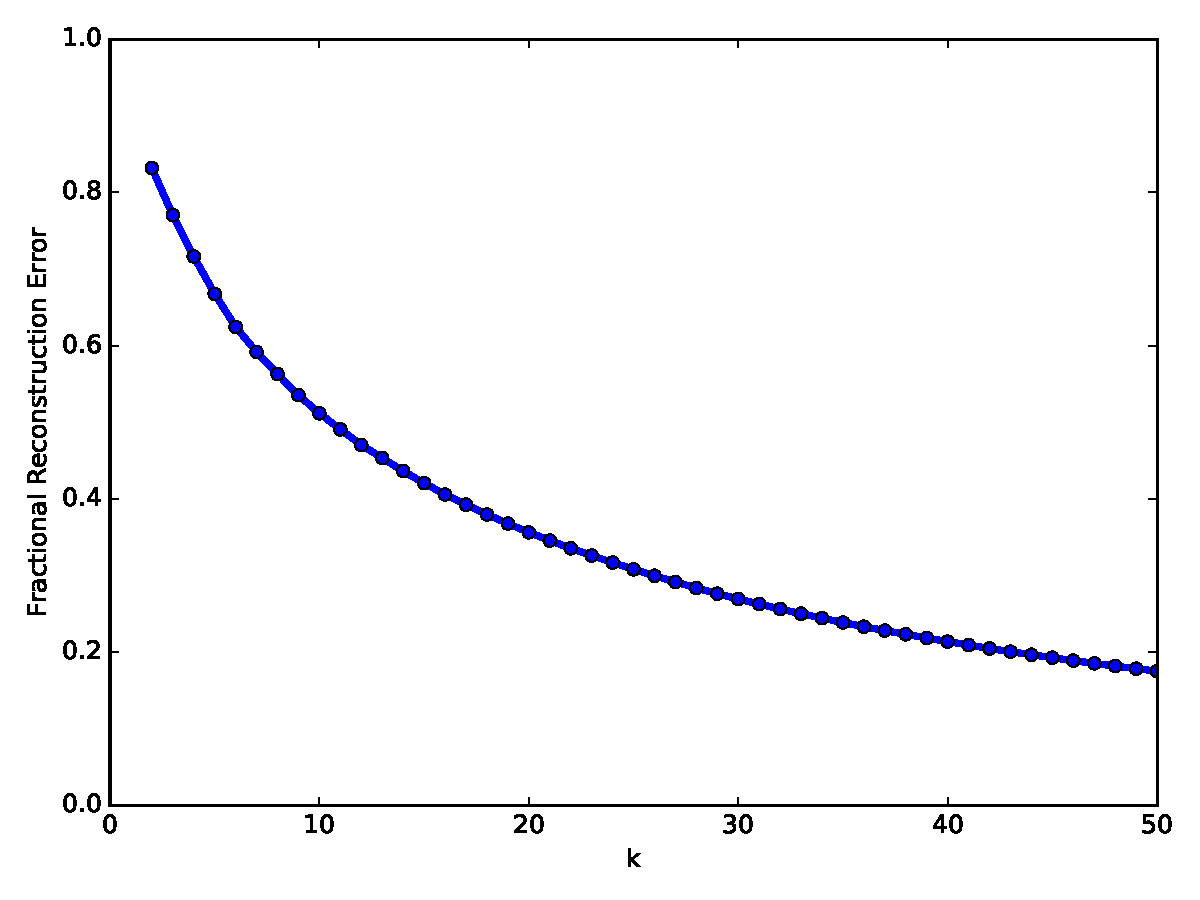
\includegraphics[width=\columnwidth]{fractional_rec_error_sans_mean.pdf}
    \caption{Fractional reconstruction error as a function of $k$ principal components out of $d$ total dimensions for $k \in [2,50]$.}
    \label{fig:frac_rec_error_sans_mean}
\end{figure}

\subsection*{1.3: Visualization of the Eigen-Directions}

\subsubsection*{1.3.1}

I plot the first 16 eigenvectors in Fig.~\ref{fig:eigendirections} as images.  To do so, I reshaped each vector into a $28 \times 28$ pixel image.  For each image, I also annotate it with its number such that the second eigendirection would have a ``2'' in its image.  I plotted 16 instead of 10 since 16 gives a nice symmetric collection of subplots.

\begin{figure}[H]
	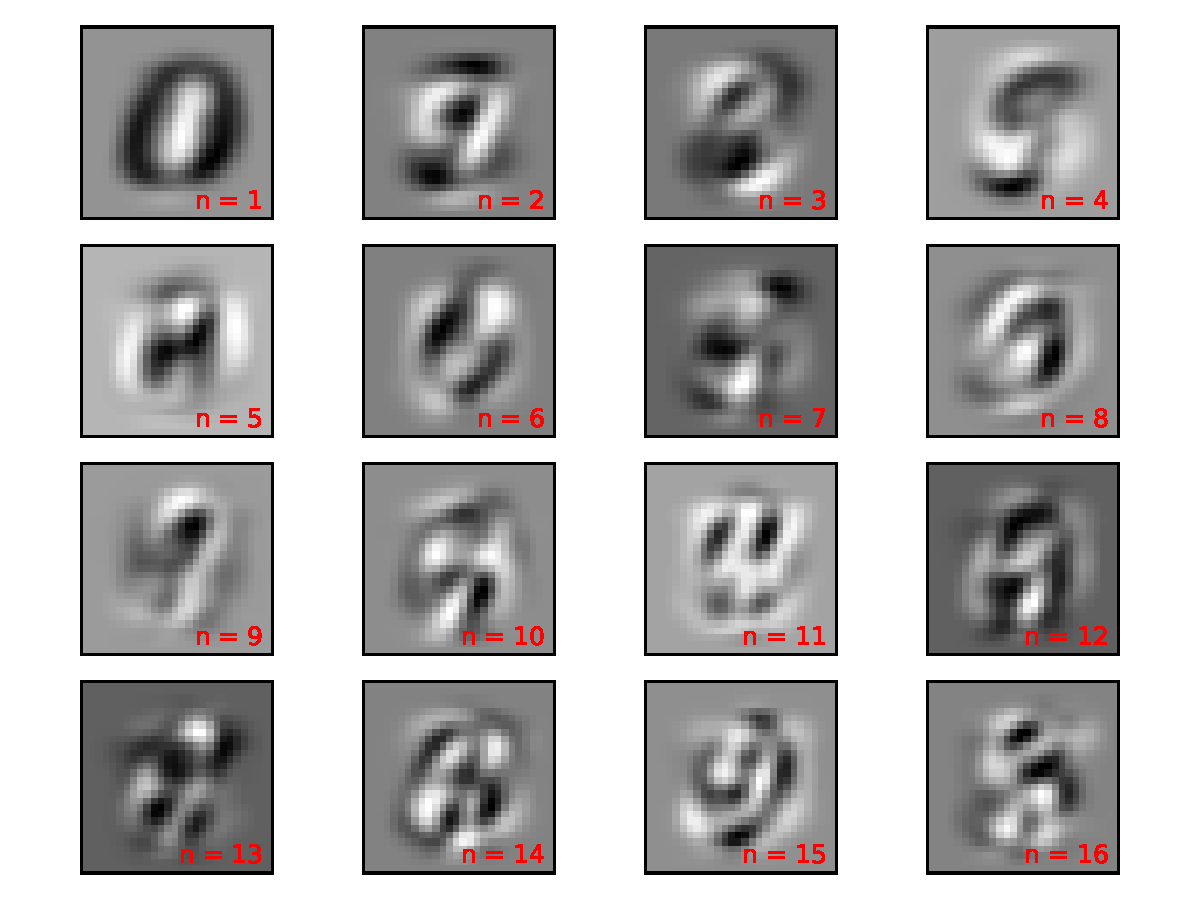
\includegraphics[width=\columnwidth]{eigendirections.pdf}
    \caption{Visualization of the first 16 eigendirections as $28 \times 28$ pixel images.  The respective eigendirection number is given in red in a subplot's lower righthand corner.}
    \label{fig:eigendirections}
\end{figure}

\subsubsection*{1.3.2}

Each individual eigendirection, or principal component, captures a fundamental basis vector in an orthogonal set which each explain a decreasing variation in the data with increasing principal component number.  That is, the first principal component accounts for the most variability in the data while subsequent components account for less and less variability.  This intuitive picture makes sense upon examining Fig.~\ref{fig:eigendirections}.  The first four components themselves appear to represent the numbers 0, 9, 3, and 5, respectively.  Although the components do not explicitly represent those numbers, instead the represent characteristics of numbers in the dataset that are commonly shared.  Many of the digits share features with 9, 3, and 5, for example, like their openings on the lefthand side of the digit and the solid vertical line on the righthand side of the digit.

\subsection*{1.4: Visualization and Reconstruction}

\subsubsection*{1.4.1}
Here, I choose 6 unique digits from the MNIST training set and plot them in Fig.~\ref{fig:mnist_digits}.  I annotate each digit's image with its label in the lower-righthand corner.  I chose 6 digits instead of 5 for symmetry's sake.
\begin{figure}[H]
	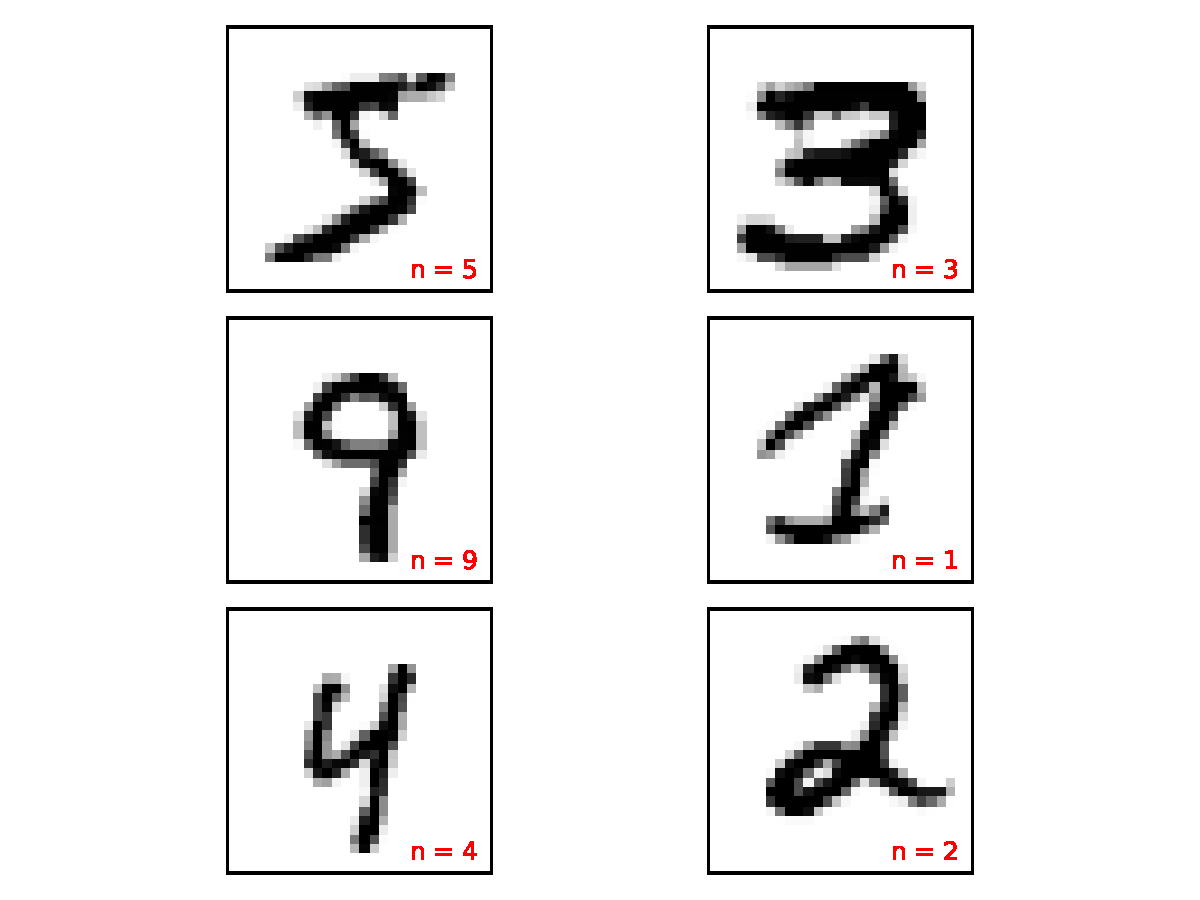
\includegraphics[width=\columnwidth]{mnist_digits.pdf}
    \caption{Visualization of 6 random, unique digits from the MNIST training set.  The image label is displayed in red in the lower-righthand corner of each image.}
    \label{fig:mnist_digits}
\end{figure}

\subsubsection*{1.4.2}

Now I perform PCA on the MNIST training set keeping the first 100 principal components.  Using this fit and the same digits displayed in Fig.~\ref{fig:mnist_digits}, I reconstruct the digits using 2, 5, 10, 20, 50, and 100 principal components using the reconstruction $X_{recon} = Xvv^T$.  The reconstructions are displayed in Fig.~\ref{fig:recon_5}, Fig.~\ref{fig:recon_3}, Fig.~\ref{fig:recon_9}, Fig.~\ref{fig:recon_1}, Fig.~\ref{fig:recon_2}, and Fig.~\ref{fig:recon_4}.  For each reconstructed image using $k$ principal components, $k$ is shown in red in the lower-righthand corner.

\begin{figure}[H]
	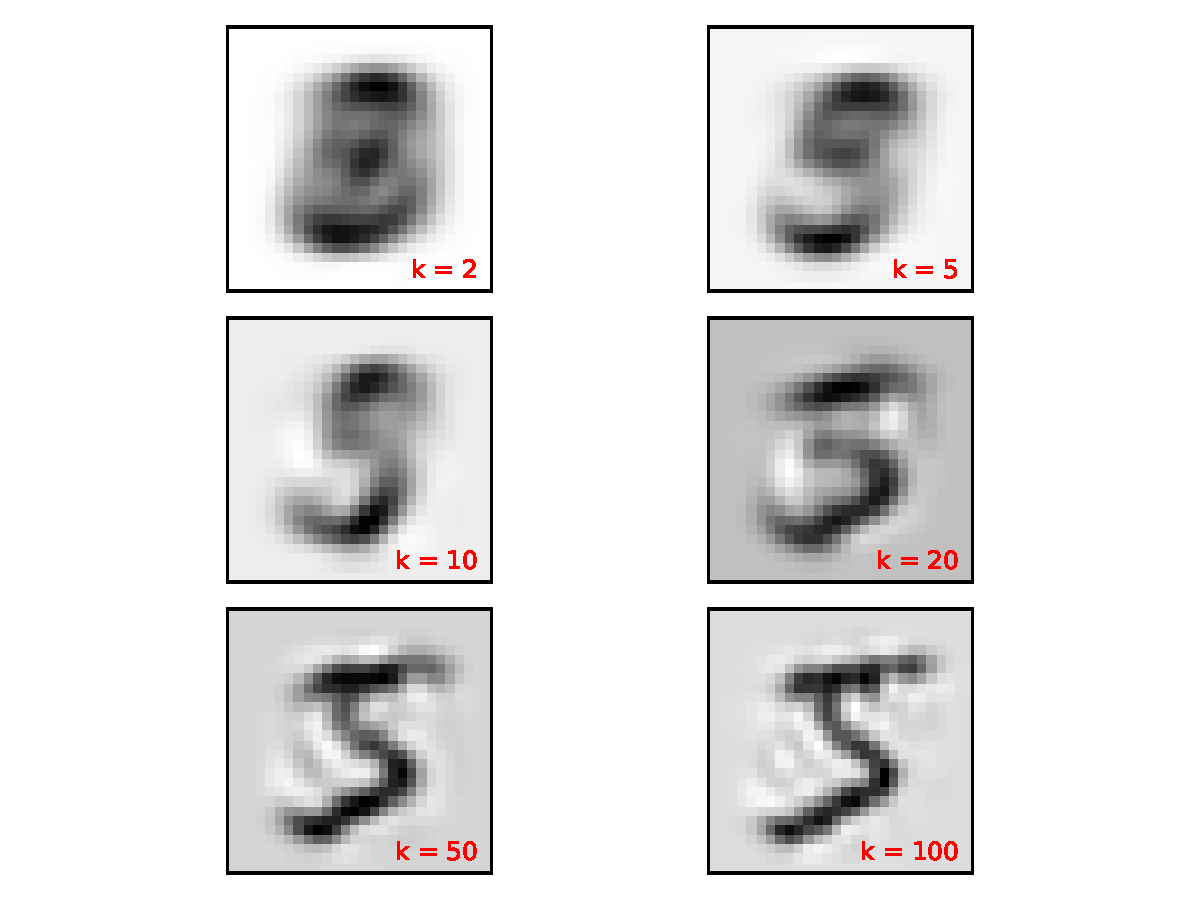
\includegraphics[width=\columnwidth]{5_recon_mnist.pdf}
    \caption{Reconstruction of a number 5 from the MNIST data set (see Fig.~\ref{fig:mnist_digits} using $k \in [2,5,10,20,50,100]$ principal components where the given $k$ is denoted in red in the lower-righthand corner of the respective subplot.}
    \label{fig:recon_5}
\end{figure}

\begin{figure}[H]
	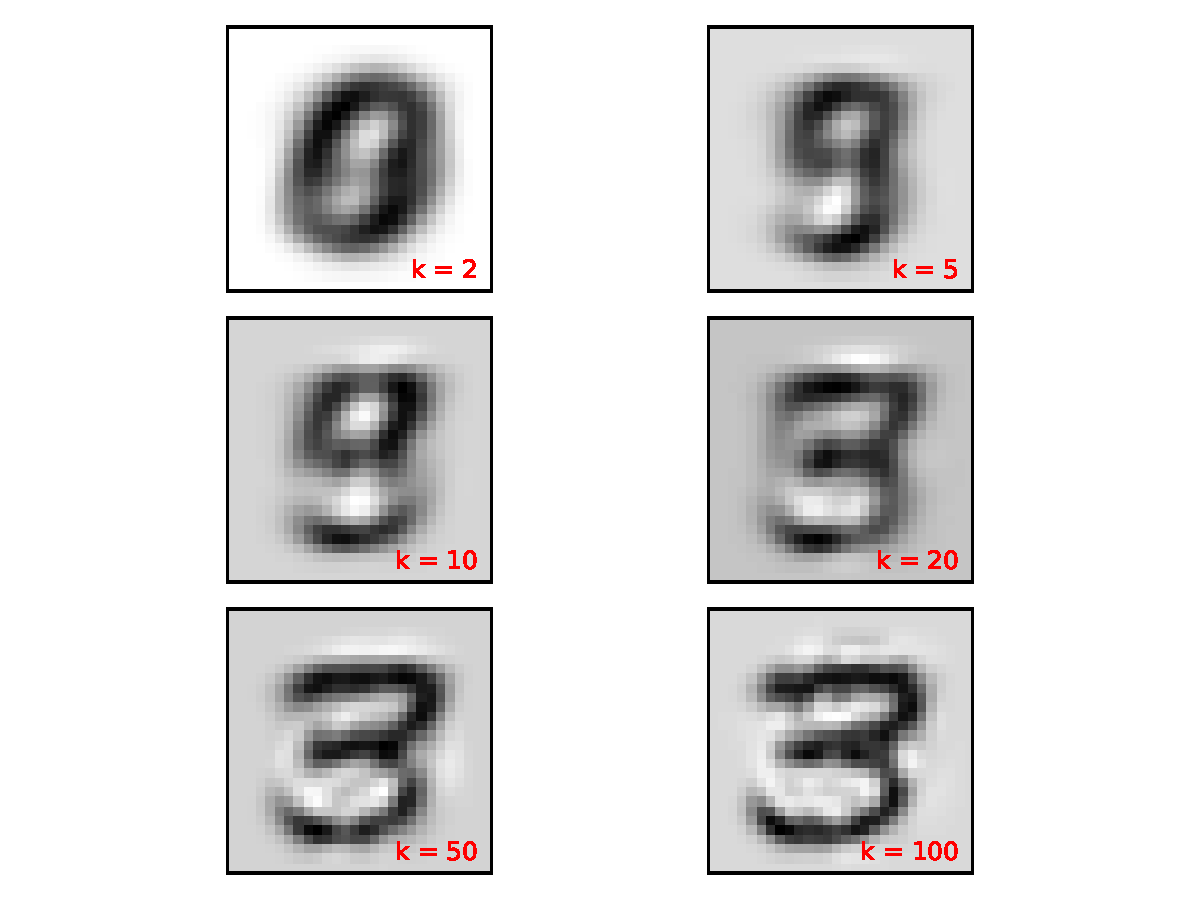
\includegraphics[width=\columnwidth]{3_recon_mnist.pdf}
    \caption{Reconstruction of a number 3 from the MNIST data set (see Fig.~\ref{fig:mnist_digits}) using $k \in [2,5,10,20,50,100]$ principal components where the given $k$ is denoted in red in the lower-righthand corner of the respective subplot.}
    \label{fig:recon_3}
\end{figure}

\begin{figure}[H]
	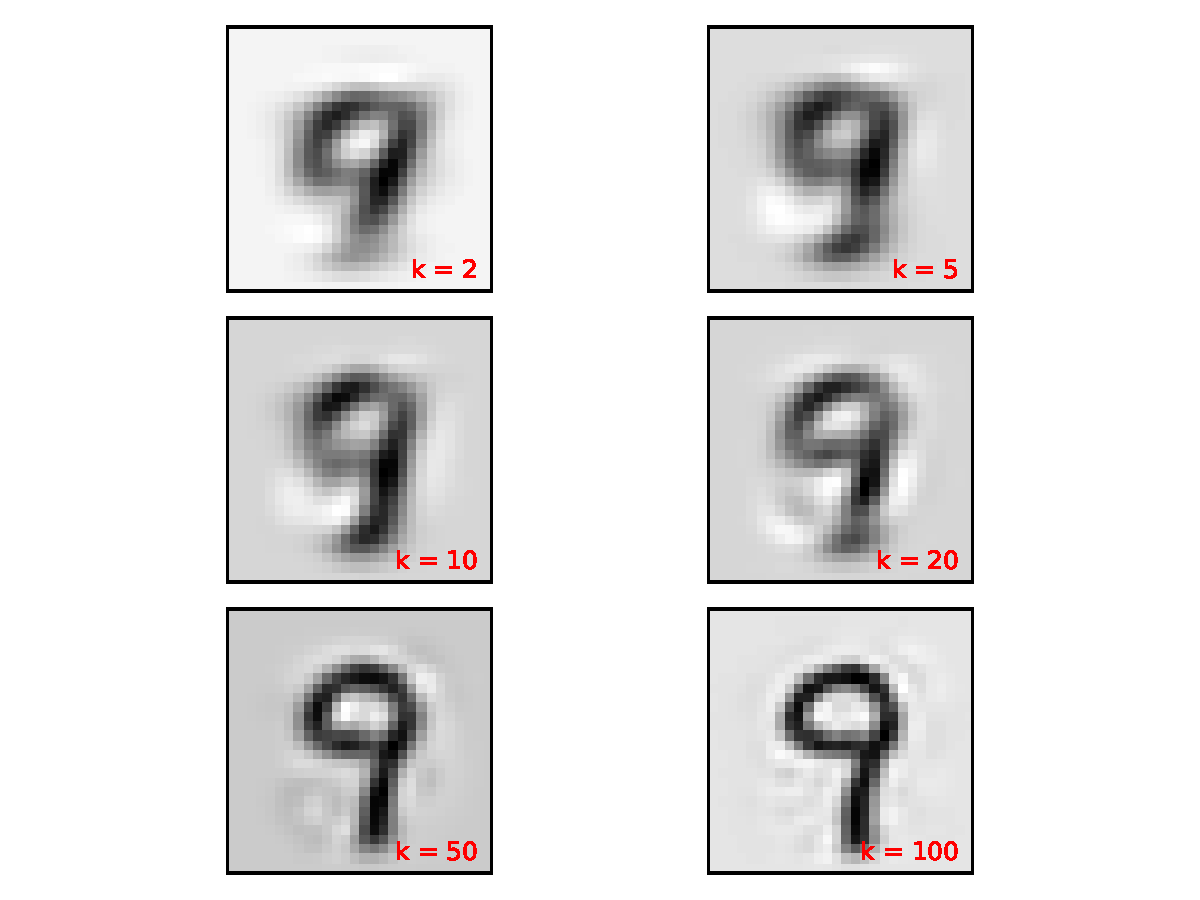
\includegraphics[width=\columnwidth]{9_recon_mnist.pdf}
    \caption{Reconstruction of a number 9 from the MNIST data set (see Fig.~\ref{fig:mnist_digits}) using $k \in [2,5,10,20,50,100]$ principal components where the given $k$ is denoted in red in the lower-righthand corner of the respective subplot.}
    \label{fig:recon_9}
\end{figure}

\begin{figure}[H]
	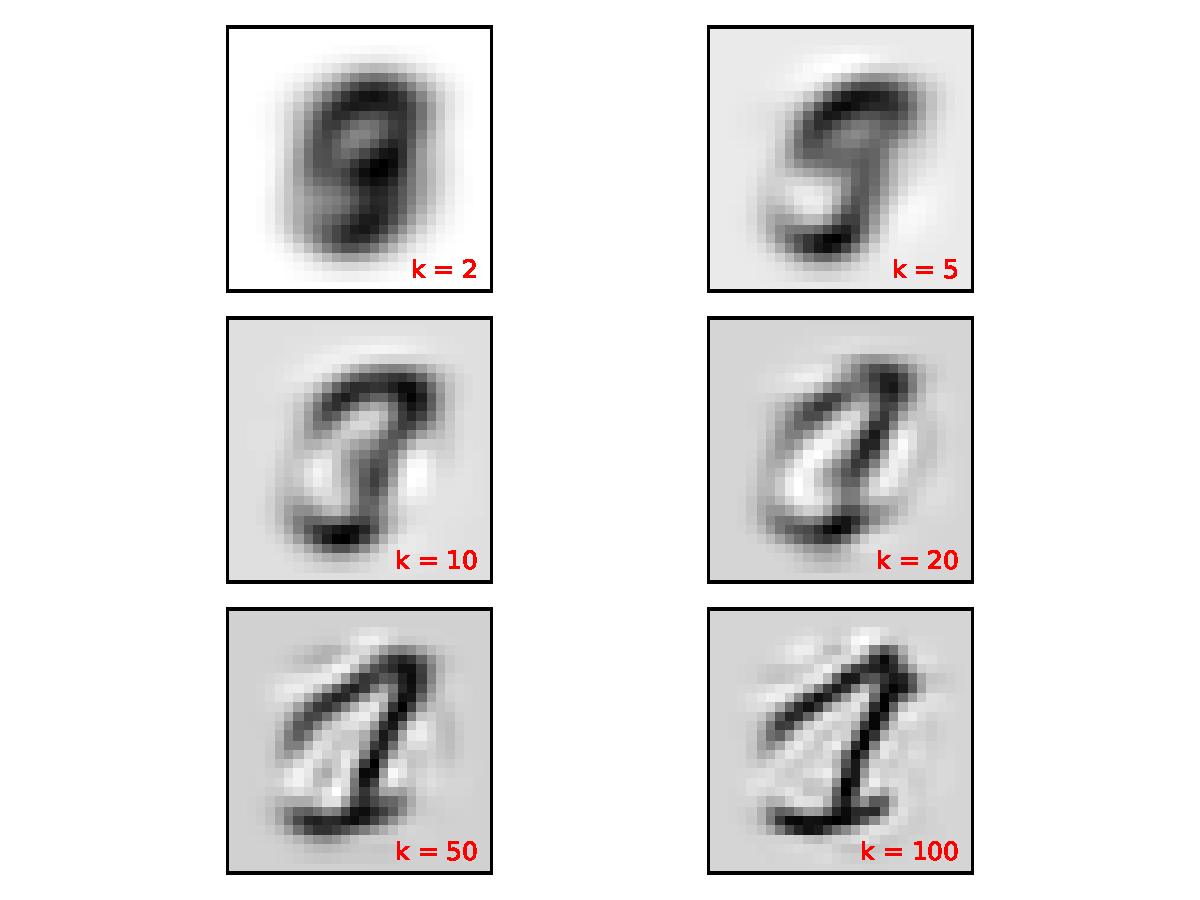
\includegraphics[width=\columnwidth]{1_recon_mnist.pdf}
    \caption{Reconstruction of a number 1 from the MNIST data set (see Fig.~\ref{fig:mnist_digits}) using $k \in [2,5,10,20,50,100]$ principal components where the given $k$ is denoted in red in the lower-righthand corner of the respective subplot.}
    \label{fig:recon_1}
\end{figure}

\begin{figure}[H]
	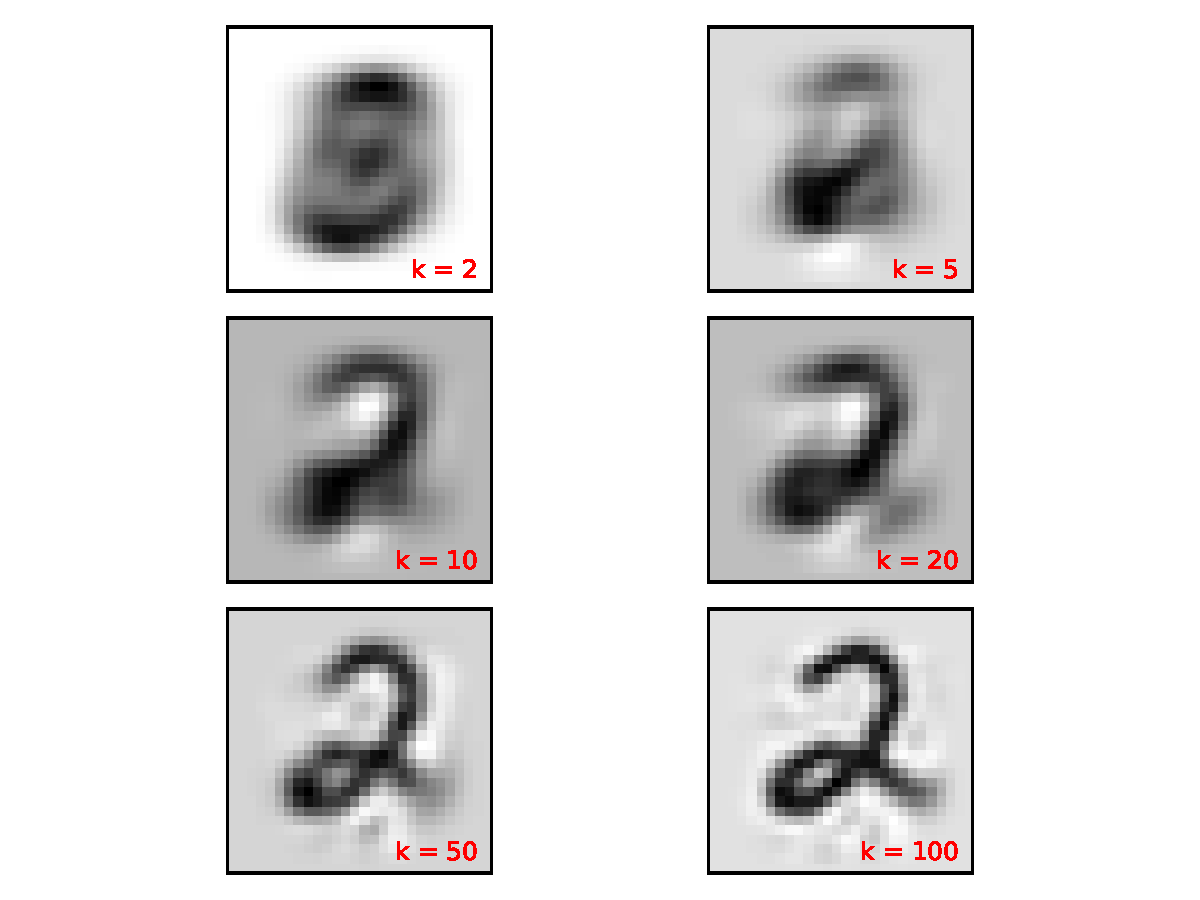
\includegraphics[width=\columnwidth]{2_recon_mnist.pdf}
    \caption{Reconstruction of a number 2 from the MNIST data set (see Fig.~\ref{fig:mnist_digits}) using $k \in [2,5,10,20,50,100]$ principal components where the given $k$ is denoted in red in the lower-righthand corner of the respective subplot.}
    \label{fig:recon_2}
\end{figure}

\begin{figure}[H]
	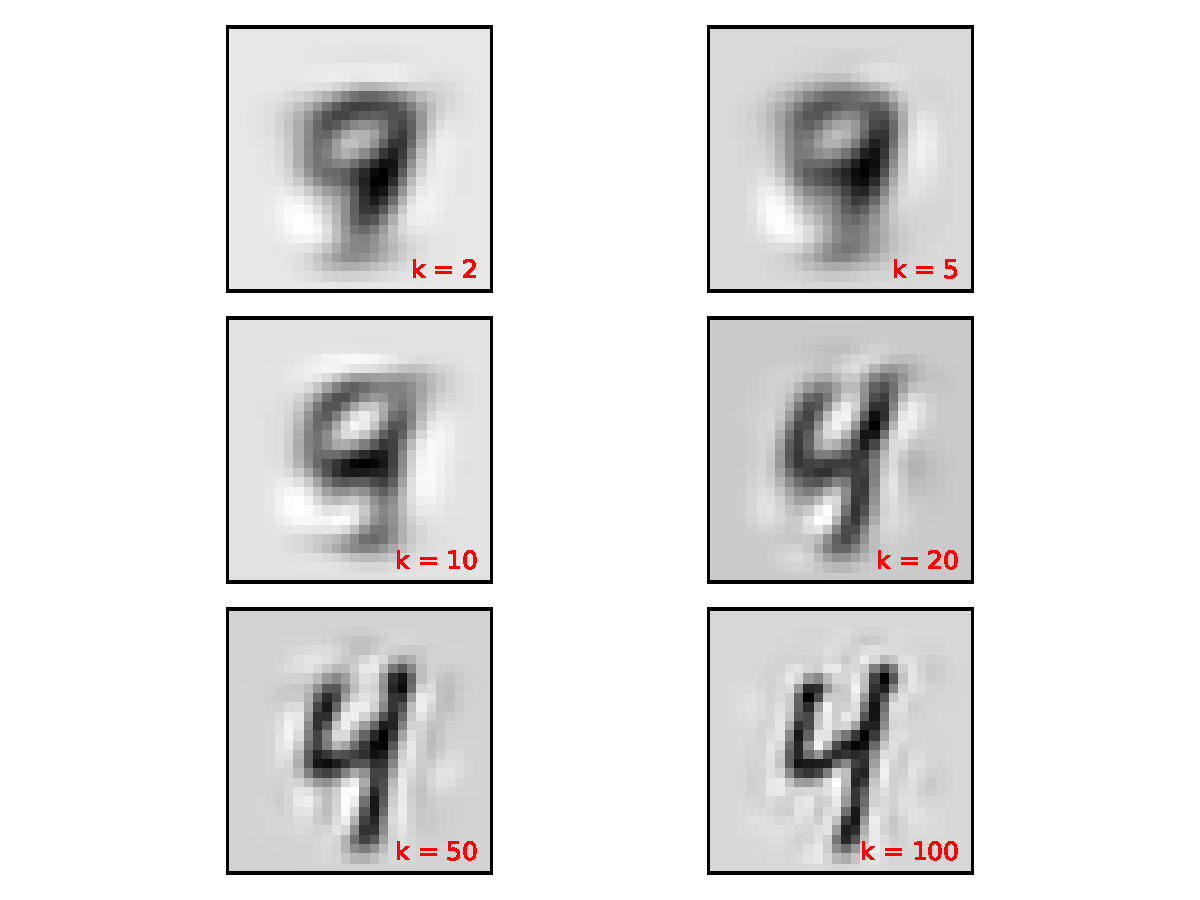
\includegraphics[width=\columnwidth]{4_recon_mnist.pdf}
    \caption{Reconstruction of a number 4 from the MNIST data set (see Fig.~\ref{fig:mnist_digits}) using $k \in [2,5,10,20,50,100]$ principal components where the given $k$ is denoted in red in the lower-righthand corner of the respective subplot.}
    \label{fig:recon_4}
\end{figure}

\subsubsection*{1.4.3}

Broadly, the images reconstructed using at least $k = 20$ principal components appear to be a good, albeit grainy, approximation of the true image.  Some images, in particular the reconstructed 9 and 5, are decently approximated using 10 principal components.  Other digits that have large scatter in how they are drawn, such as 4s, require more principal components to adequately approximate the true image.  All digits reconstructed with at least 50 principal components are good approximations of the original images.  As expected, the more principal components used, the better the approximation becomes since as $k \rightarrow d$, we expect the reconstruction to become equal to the original $X$.

\section*{2: Let's get to state of the art of MNIST!}

In this section, I use one-against least-squares classification to attempt to get to ``state of the art" on the MNIST dataset.  The code used to solve this question is in the following attached files: {\tt hw3$\_$2.py} in the {\tt HW3} directory and {\tt pca/pca.py, regression/regression$\_$utils.py, validation/validation.py, data$\_$processing/mnist$\_$utils.py, optimization/gradient$\_$descent.py, kernel/kernel.py} all in the {\tt DML} directory.

\subsection*{2.1 Least Squares}

For computational speed purposes, I first performed dimension reduction using PCA.  I fit my PCA algorithm on the MNIST training set with the mean subtracted out then projected each image using the first $k = 50$ components.  I mapped the $n \times k$ reduced MNIST training data for $n$ samples to a $n \times n$ transformed MNIST training set using a random Fourier feature approximation of an RBF kernel of the form
\begin{equation} \label{eqn:rbf_kernel}
h_j(x) = \sin \left( \frac{v_i \cdot x}{\sigma} \right)
\end{equation}
where $h_j(x)$ is the $jth$ feature out of $n$ of the transformed image $x$.  The transformation matrix $v$ is composed of $k = 60,000$ columns where each coordinate of the $k$ columns are independently sampled from the standard normal distribution.  The same matrix $v$ was used to transform both the training and testing sets.  I selected the bandwidth $\sigma$ by taking the mean of the pairwise distance of about 100 samples and scaling that value by TODO.  I explored several other values for $\sigma$, TODO, TODO, ..., and TODO and found that TODO yielded the best performance.  

Since the transformed training data matrix was so large, I used mini-batch SGD with a mini-batch size of 100 for all gradient calculations.  Each epoch, or each complete pass through a randomly permuted training set, I performed 60,000/100 = 600 mini-batch gradient updates.  I computed the loss of the entire transformed training set and testing set (to which I applied the same transformation as the training set for consistency).  In addition over a given epoch, I averaged the weight vectors and offset terms to get $\bar{w}$ and $\bar{w}_0$ and used these to compute losses as well.  I called my algorithm converged once the mean square loss on the training set did not change by more than $0.1\%$ (TODO).  I did not explicitly use regularization since the early-stopping from my learning rate decay scheme (described below) and my convergence criterion implicitly $l_2$ regularize my solution.

\subsubsection*{2.1.1}

I used a learning rate $\eta = 2 \times 10^{-5}$ as gave the best fit.  In practice in my SGD implementation at the start of each epoch, I reset $\eta = k\eta_0/N$ where $N$ is the number of samples in a batch, $k = 1/\sqrt{t}$ is a scaling constant where $t$ is the epoch number and $\eta_0 = 2 \times 10^{-5}$.  I used a mini-batch size of 100 and a kernel bandwidth of TODO computing using the scheme described above.

\subsubsection*{2.1.2}

\begin{figure}[H]
	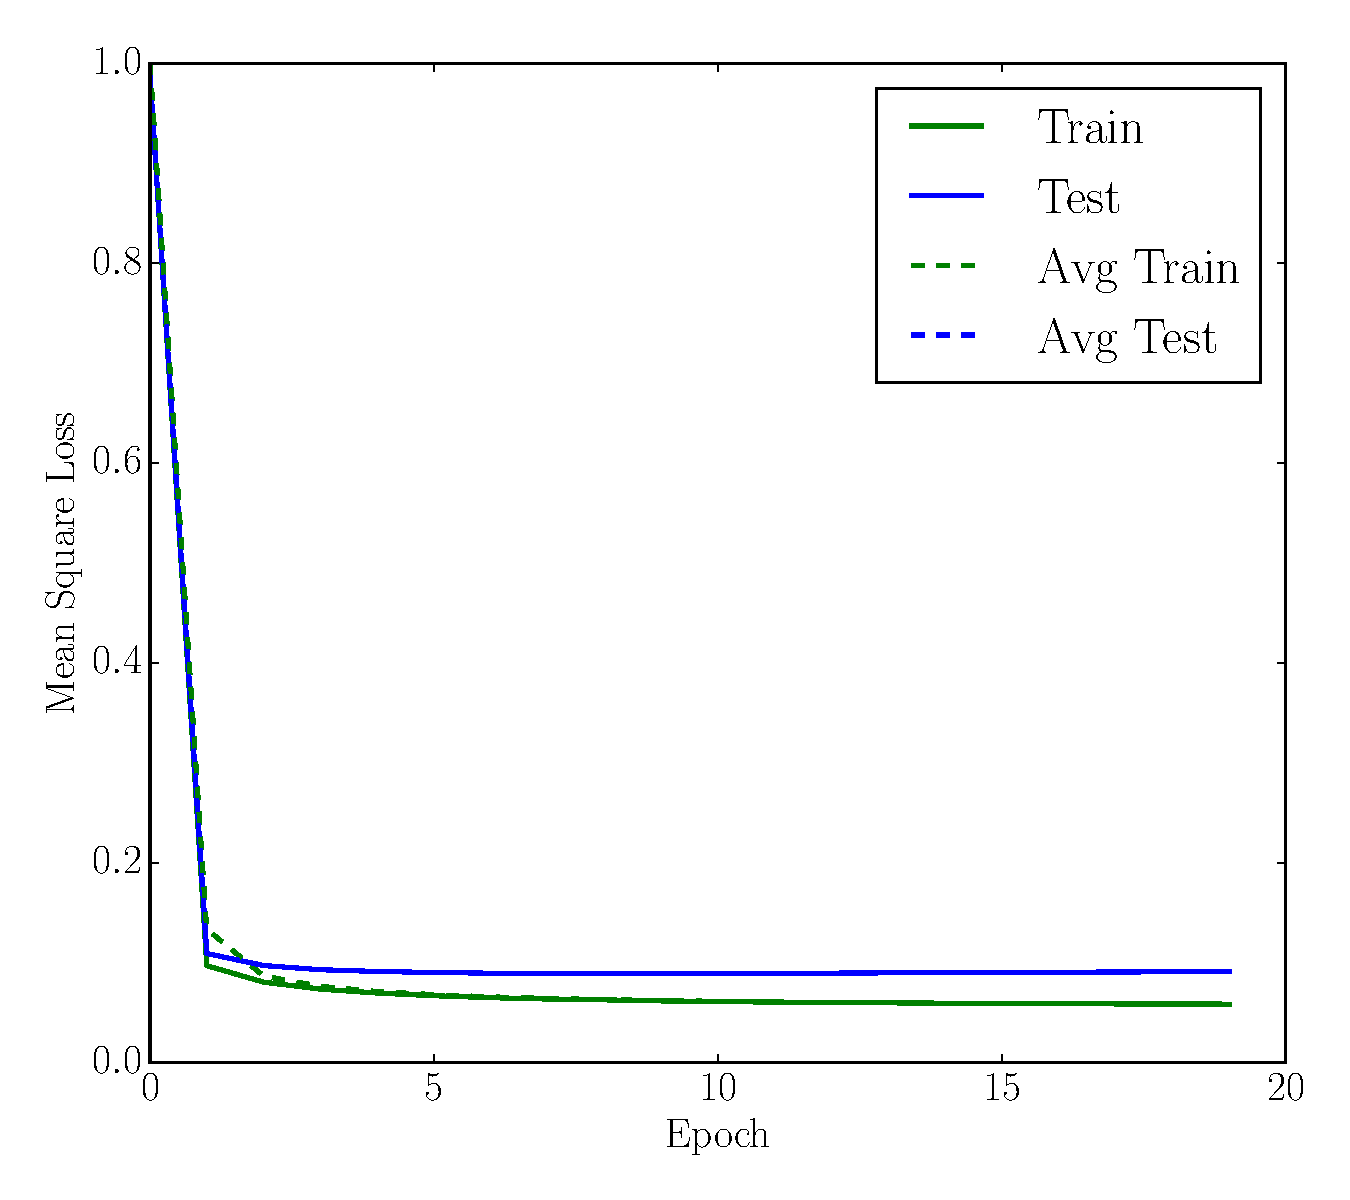
\includegraphics[width=\columnwidth]{pca_square_loss.pdf}
    \caption{Mean square loss versus epoch for the both the MNIST training and testing sets for both the $w_t$ and $\bar{w}_{\tau}$. Note that the curves for the training and testing errors overlap.}
    \label{fig:pca_square_loss}
\end{figure}

TODO description

\subsubsection*{2.1.3}

\begin{figure}[H]
	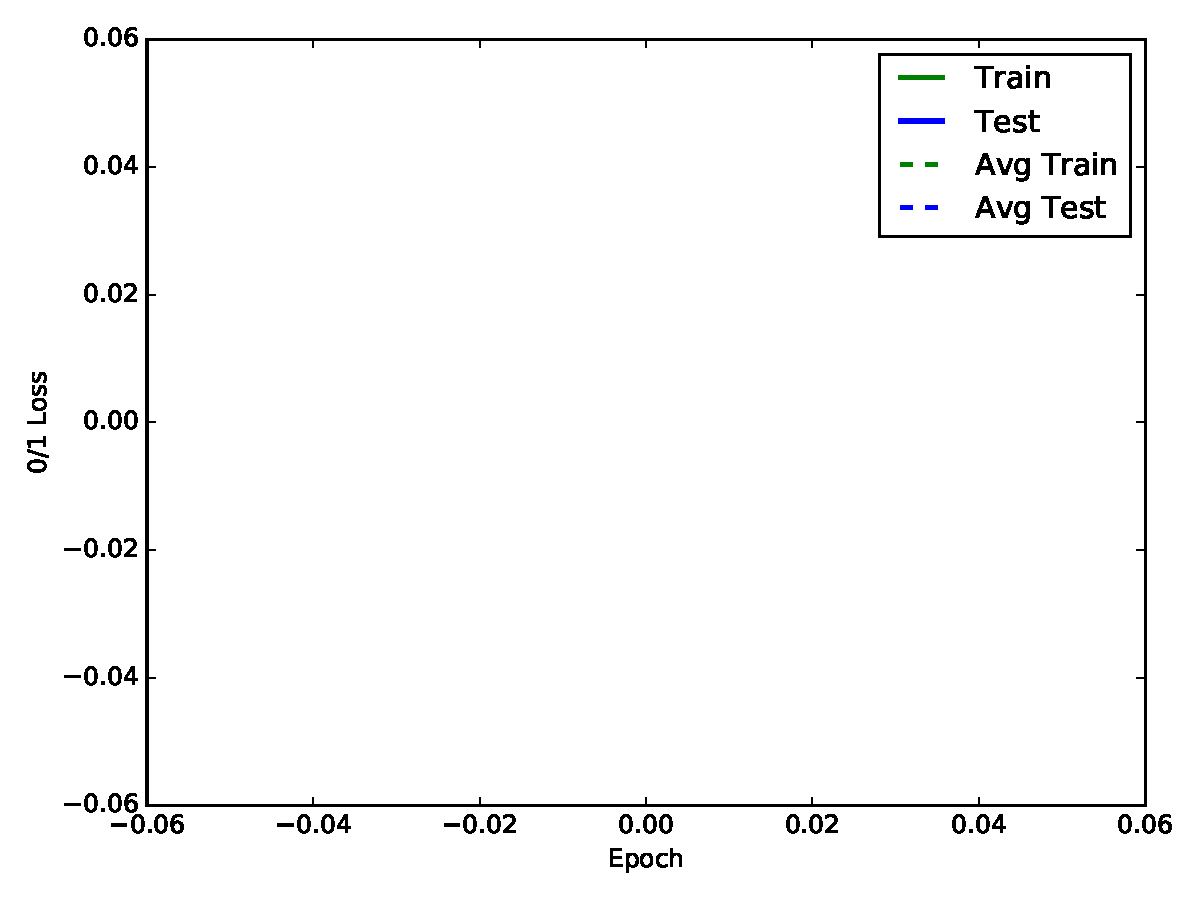
\includegraphics[width=\columnwidth]{pca_01_loss_masked.pdf}
    \caption{0/1 loss versus epoch for the both the MNIST training and testing sets for both the $w_t$ and $\bar{w}_{\tau}$ computed after the testing loss dipped below $5\%$.}
    \label{fig:pca_01_loss_masked}
\end{figure}

TODO description

\subsubsection*{2.1.4}

The final training squared loss and 0/1 loss are TODO and TODO, respectively.  The total number of mistakes made on the training set of the final point are TODO.  The same values computed using $\bar{w}_{\tau}$ are TODO, TODO, and TODO.

\subsubsection*{2.1.5}

The final testing squared loss and 0/1 loss are TODO and TODO, respectively.  The total number of mistakes made on the testing set of the final point are TODO.  The same values computed using $\bar{w}_{\tau}$ are TODO, TODO, and TODO.

\subsection*{2.2: EXTRA CREDIT: Softmax Classification}

\subsubsection*{2.2.1}

I used a learning rate $\eta = 2 \times 10^{-5}$ as gave the best fit.  In practice in my SGD implementation at the start of each epoch, I reset $\eta = k\eta_0/N$ where $N$ is the number of samples in a batch, $k = 1/\sqrt{t}$ is a scaling constant where $t$ is the epoch number and $\eta_0 = 2 \times 10^{-5}$.  I used a mini-batch size of 100 and a kernel bandwidth of TODO computing using the scheme described above.

\subsubsection*{2.2.2}

\begin{figure}[H]
	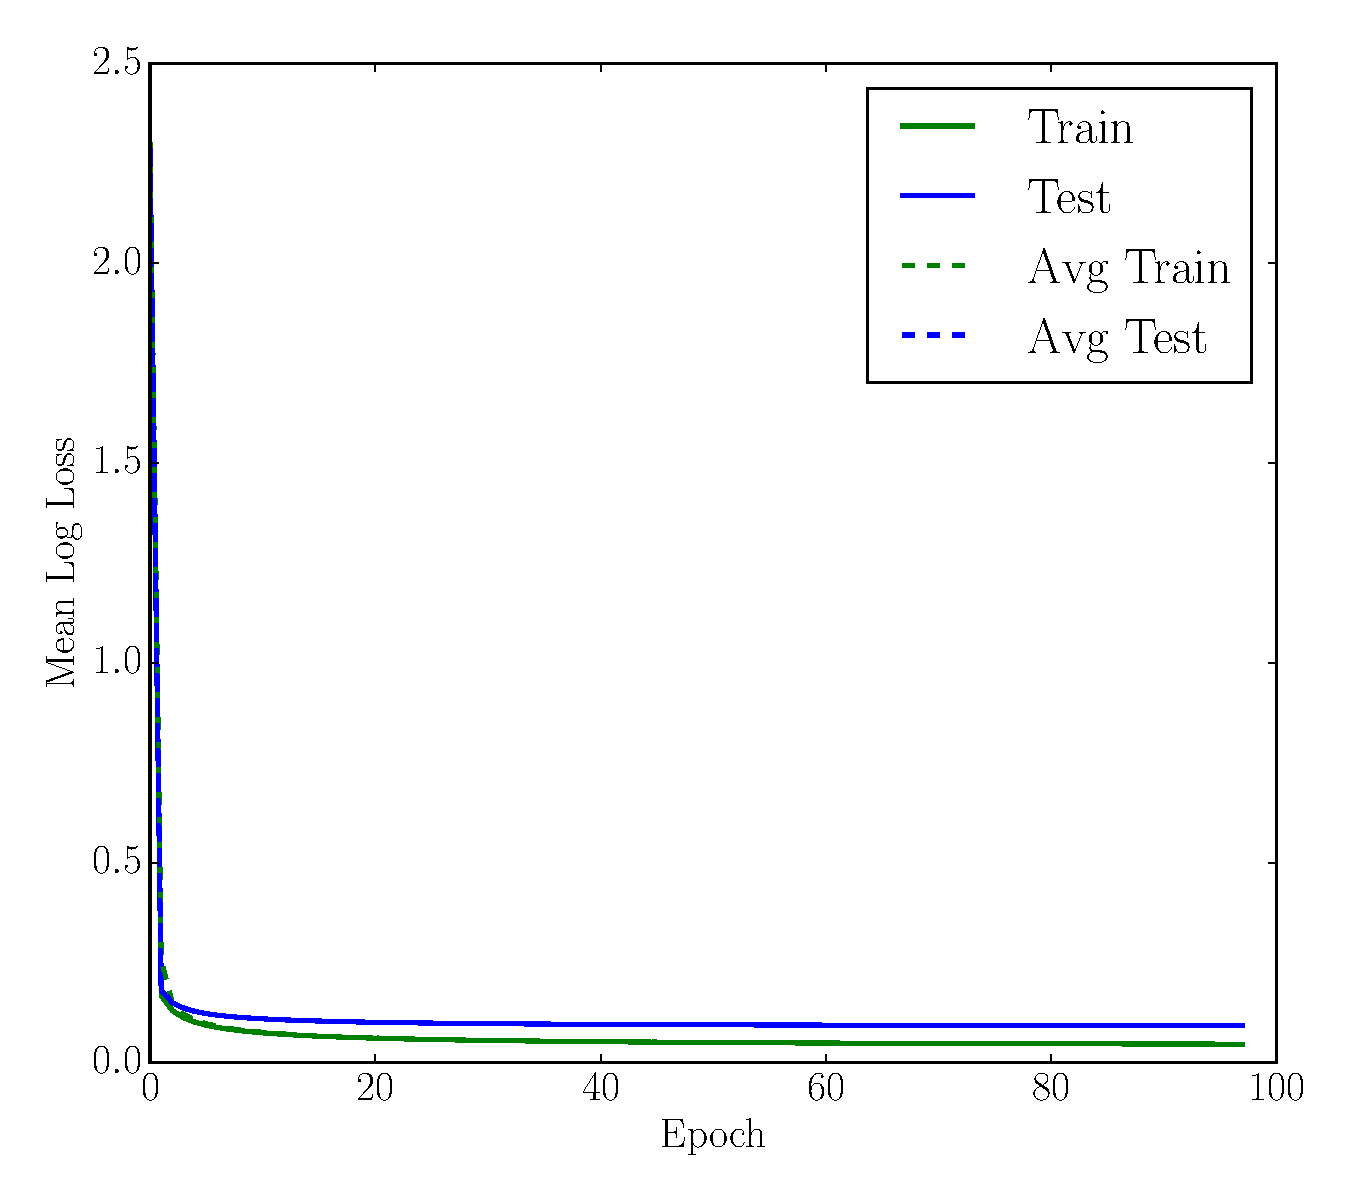
\includegraphics[width=\columnwidth]{logistic_log_loss.pdf}
    \caption{Mean log loss versus epoch for the both the MNIST training and testing sets for both the $w_t$ and $\bar{w}_{\tau}$.}
    \label{fig:logistic_log_loss}
\end{figure}

TODO description

\subsubsection*{2.2.3}

\begin{figure}[H]
	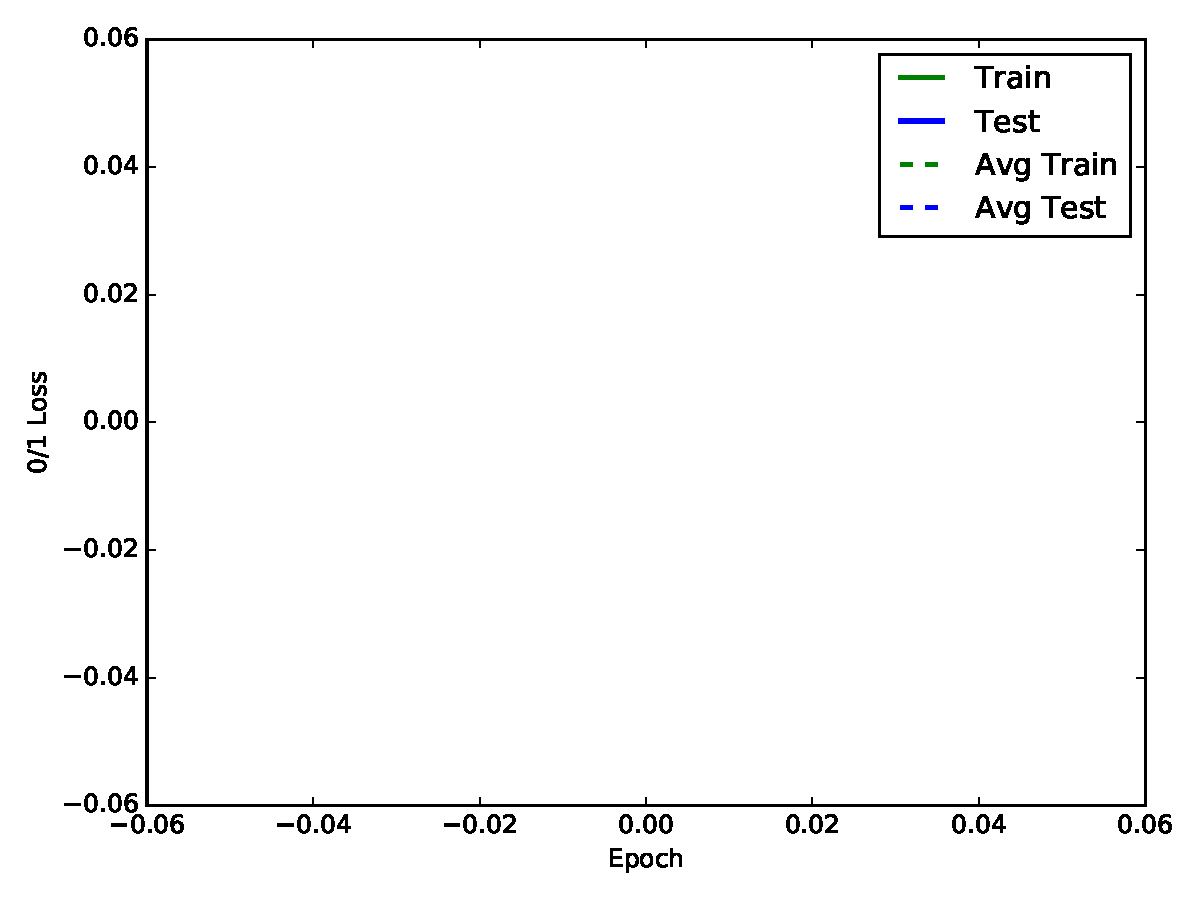
\includegraphics[width=\columnwidth]{logistic_01_loss_masked.pdf}
    \caption{0/1 loss versus epoch for the both the MNIST training and testing sets for both the $w_t$ and $\bar{w}_{\tau}$ computed after the testing loss dipped below $5\%$.}
    \label{fig:logistic_01_loss_masked}
\end{figure}

TODO description

\subsubsection*{2.2.4}

The final training log loss and 0/1 loss are TODO and TODO, respectively.  The total number of mistakes made on the training set of the final point are TODO.  The same values computed using $\bar{w}_{\tau}$ are TODO, TODO, and TODO.

\subsubsection*{2.2.5}

The final testing log loss and 0/1 loss are TODO and TODO, respectively.  The total number of mistakes made on the testing set of the final point are TODO.  The same values computed using $\bar{w}_{\tau}$ are TODO, TODO, and TODO.

\section*{3: SVMs: Hinge loss and mistake bounds}

Here, I work with a SVM which classifies according to the hypothesis:
\begin{equation} \label{eqn:svm}
h_w(x) = \text{sgn}(w^Tx)
\end{equation}
and the SVM loss function, the hinge loss, is given by
\begin{equation} \label{eqn:hinge_loss}
l((x,y),w) = \max(0,1 - yw^Tx)
\end{equation}
for $y \in [-1,1]$.

\subsection*{3.1}

I can show that a function is convex if it is lower-bounded by its gradient (or subgradient, more generally).  Here, I will examine the $y = 1$ case since the $y = -1$ case proceeds analogously.   For the $w^Tx > 1$ case, Eqn.~\ref{eqn:hinge_loss} gives 0.  The gradient with respect to $w$ in this regime is 0 and lower-bounds then function.  When $w^Tx < 1, w^Tx \neq 0$, the gradient with respect to $w$ in this regime is $X$.  Since this is linear and $w^TX$, is linear with $w$, its gradient lower bounds it.  Finally when $w^Tx = 1$, the hinge point, the derivative is undefined so instead I use a subgradient.  For the subgradient, it can be anything tangent line with slope between $[0,X]$, so I will use 0 for simplicity.  This too lower bounds the function.  Since the function is lower-bounded by its (sub)gradient at all points, it is convex.  A similar argument applies for the $y = -1$ case.

\subsection*{3.2}

For a correct prediction, $y_i = \text{sgn}(w^Tx_i)$ holds.  Here, I will just consider the $y = 1$ case for simplicity since the $y = -1$ case proceeds analogously.  Here, the hinge loss is given as $HL = \max(0,1-w^TX)$.  Since $w^TX < 0$ cannot hold when $y_i = 1 = \text{sgn}(w^Tx_i)$, I will not consider it.  If $w^TX = 0$, then the hinge loss is 1.  If $w^TX \geq 1$, the hinge loss is 0.  Therefore for correct predictions, the hinge loss ranges from $HL \in [0,1]$.

\subsection*{3.3}

Define the mistake bound as
\begin{equation} \label{eqn:mistake_bound}
\frac{1}{n}M(w) \leq \frac{1}{n}\sum_{i = 1}^n \max(0, 1 - y_i w^T x_i)
\end{equation}
where in my proof I will ignore the $1/n$ factor since it is merely a normalization term.  If you consider the two regimes where your predictions are incorrect and correct, Eqn.~\ref{eqn:mistake_bound} becomes
\begin{equation} \label{eqn:mb} 
M(w) \leq \sum_{w^Tx_i \in \text{correct}} \max(0, 1 - y_i w^T x_i) + \sum_{w^Tx_i \in \text{incorrect}} \max(0, 1 - y_i w^T x_i).
\end{equation}

The sum over the correct predictions will always be $\geq 0$ since in the above question I showed that the hinge loss ranges from $[0,1]$ for correct predictions.  The sum over incorrect predictions will be at least to $M(w)$ since for the hinge loss for an incorrect prediction, the best you can do is 1 when $w^Tx = 0$.  Therefore if all your all your incorrect predictions are these ``best" incorrect predictions, the sum over all incorrect predictions will be $M(w)$, giving you the stated lower bound and proving Eqn.~\ref{eqn:mistake_bound}.  

\section*{4: Fitting an SVM classifier by hand}

TODO

\subsection*{4.1}

TODO

\subsection*{4.2}

TODO

\subsection*{4.3}

TODO

\subsection*{4.4}

TODO

\subsection*{4.5}

TODO

\section*{5: K-Means}

In this question, I implement the K-means clustering algorithm and apply it to the MNIST dataset.  The code used to solve this question is in the following attached files: {\tt hw3$\_$5.1.py, hw3$\_$5.2.py} in the {\tt HW3} directory and {\tt clustering/kmeans.py, validation/validation.py, data$\_$processing/mnist$\_$utils.py} in the {\tt DML} directory.

\subsection*{5.0: K-Means Algorithm Implementation}

My K-means algorithm follows the algorithm presented in the Murphy textbook.  First, I initialize my $k$ clusters using $k$ random samples from the MNIST training set to make a $k \times d$ cluster matrix $\mu$ for $d$ features.  Each iteration, I perform the following E and M steps.  In the E step, I assign a label $z$ to each sample $X_i$ subject to
\begin{equation} \label{eqn:E_step}
z_i = \text{argmin}_k ||X_i - \mu_k ||_2^2
\end{equation}
which assigns a point $X_i$ to the closest cluster center $\mu_k$ according to the squared Euclidean distance.  After passing through the training set and assigning each point to its nearest cluster center, I perform the M step in which I calculate the new cluster centers to be the centroids of the samples in each cluster as follows
\begin{equation} \label{eqn:M_step}
\mu_k = \frac{1}{N_k} \sum_{i = 1}^{N_k} X_i
\end{equation}
where there are $N_k$ samples in the $kth$ cluster.  I call the algorithm converged once all the samples' labels no longer change.

\subsection*{5.1: Run the algorithm}

I ran the K-means algorithm with $k = 16$ on the full MNIST training set.  As stated above, I initialized my centers $\mu_k$ using $k$ random samples from the training set.

\subsubsection*{5.1.1a}

In Fig.~\ref{fig:k_16_rec_err}, I plot the squared reconstruction error versus iteration number for $k = 16$ clusters.  I compute the squared reconstruction error as
\begin{equation} \label{eqn:sq_rec_err}
\text{SRE} = \frac{1}{N} \sum_{j = 1}^k\sum_{X_i \in \mu_j} || X_i - \mu_j ||_2^2
\end{equation}
where $\mu_j$ is the cluster $X_i$ belongs to.

\begin{figure}[H]
	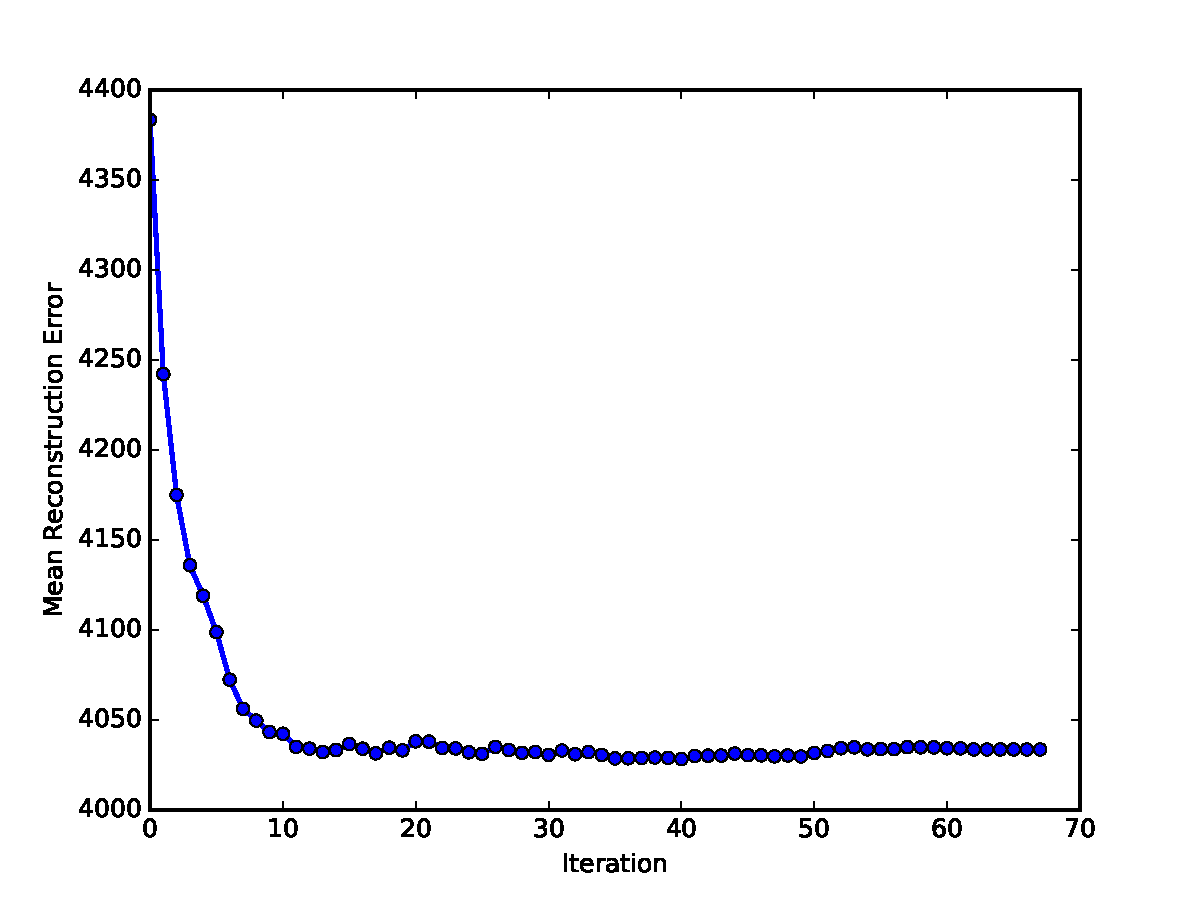
\includegraphics[width=\columnwidth]{k_16_rec_err.pdf}
    \caption{Squared reconstruction error versus iteration number for $k = 16$ clusters.}
    \label{fig:k_16_rec_err}
\end{figure}

The mean squared reconstruction error reaches near its local minimum after about 10 iterations and does not change significantly over the next 60 iterations it takes the algorithm to converge.  The final 60 or so iterations likely involved just a few points flipping labels, explaining why the error did not change appreciably.

\subsubsection*{5.1.1b}

Let us define the number of assignments for a mean to be the number of samples assigned to that mean's cluster.  In Fig.~\ref{fig:k_16_num_assignments}, I plot the number of assignments per cluster for $k = 16$ clusters ordered in descending order.

\begin{figure}[H]
	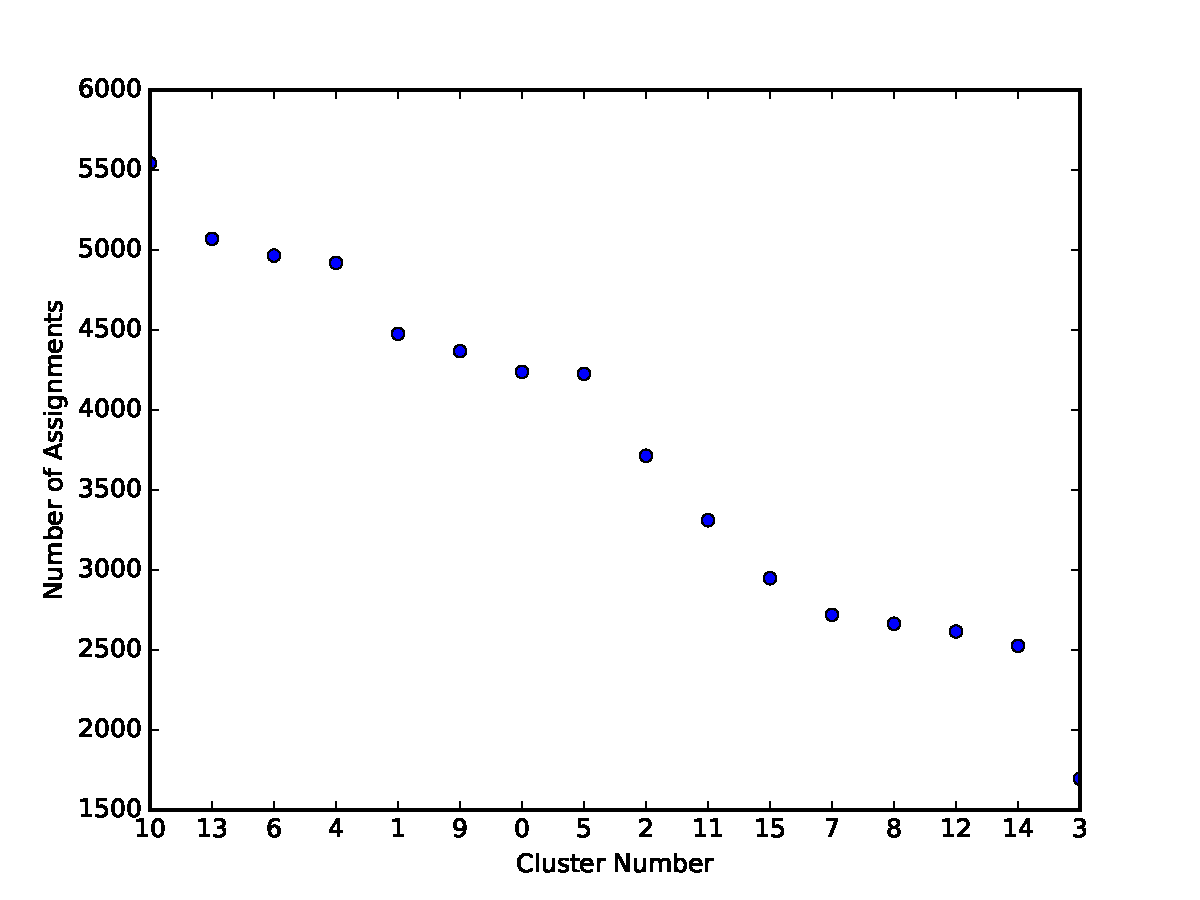
\includegraphics[width=\columnwidth]{k_16_num_assignments.pdf}
    \caption{Number of assignments per cluster for $k = 16$ clusters ordered in descending order.}
    \label{fig:k_16_num_assignments}
\end{figure}

As can be seen in the above figure, cluster 10 contains the most members at about 5,500 while cluster 3 contains the least with around 1,750 members.  I note that cluster number does not in general equal the MNIST digit label.

\subsubsection*{5.1.1c}

In Fig.~\ref{fig:k_16_means}, I visualize the $k = 16$ centers my K-means algorithm learned on the MNIST training set in descending order for number of assignments.

\begin{figure}[H]
	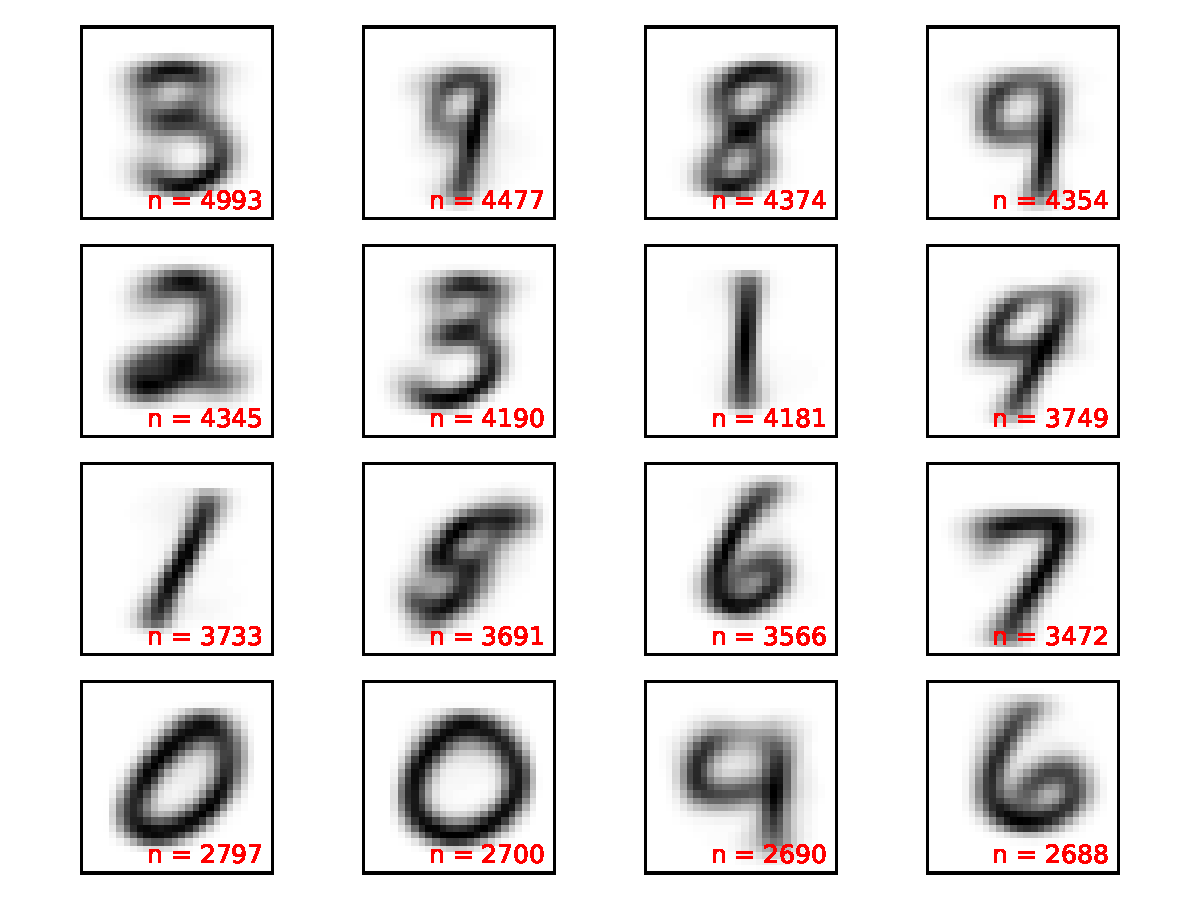
\includegraphics[width=\columnwidth]{k_16_means.pdf}
    \caption{Visualization of the $k = 16$ centers orders by number of members.  The number of members for each center is shown in each respective center's subplot in red in the lower-righthand corner.}
    \label{fig:k_16_means}
\end{figure}

\subsubsection*{5.1.2}

For my $k = 16$ cluster visualization, I find it interesting that all 10 digits are not represented amongst the 16 cluster centers.  Instead, there appears to be two classes of clusters: some that are different rotations or transformations of a given digit or some that are amalgamations of similar digits.  For example, there are several ``6"s in the clusters that are rotations or transformations of a 6, and similarly for 1s and 0s.  On the other hand, some cluster centers look like combinations of digits, such as combinations of 3s and 5s and combinations of 4s and 9s.  These behaviors make sense because of the inherent variance in how people write digits.  Not all digits are written in the same orientation or with the same curvature at certain parts of the digit causing some to look like others.

I ran the K-means algorithm with $k = 250$ on the full MNIST training set.  As stated above, I initialized my centers $\mu_k$ using $k$ random samples from the training set.

\subsubsection*{5.1.2a}

In Fig.~\ref{fig:k_250_rec_err}, I plot the squared reconstruction error versus iteration number for $k = 250$ clusters.  I compute the squared reconstruction error as in Eqn.~\ref{eqn:sq_rec_err}.
\begin{figure}[H]
	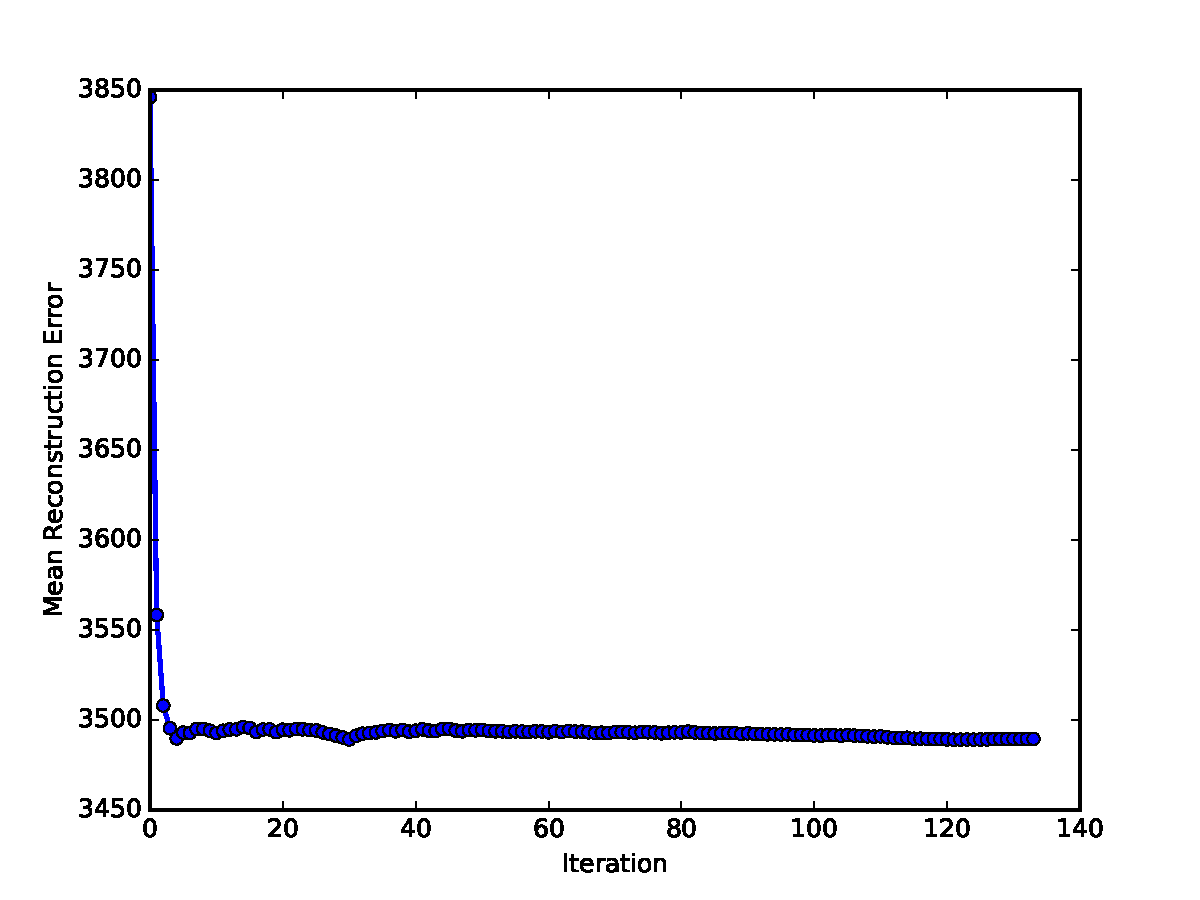
\includegraphics[width=\columnwidth]{k_250_rec_err.pdf}
    \caption{Squared reconstruction error versus iteration number for $k = 250$ clusters.}
    \label{fig:k_250_rec_err}
\end{figure}

The mean squared reconstruction error reaches near its local minimum after about 5 iterations and does not change significantly over the next 125 iterations it takes the algorithm to converge.  The final 125 or so iterations likely involved just a few points flipping labels, explaining why the error did not change appreciably and slowly decreased.

\subsubsection*{5.1.2b}

In Fig.~\ref{fig:k_250_num_assignments}, I plot the number of assignments per cluster for $k = 250$ clusters ordered in descending order.

\begin{figure}[H]
	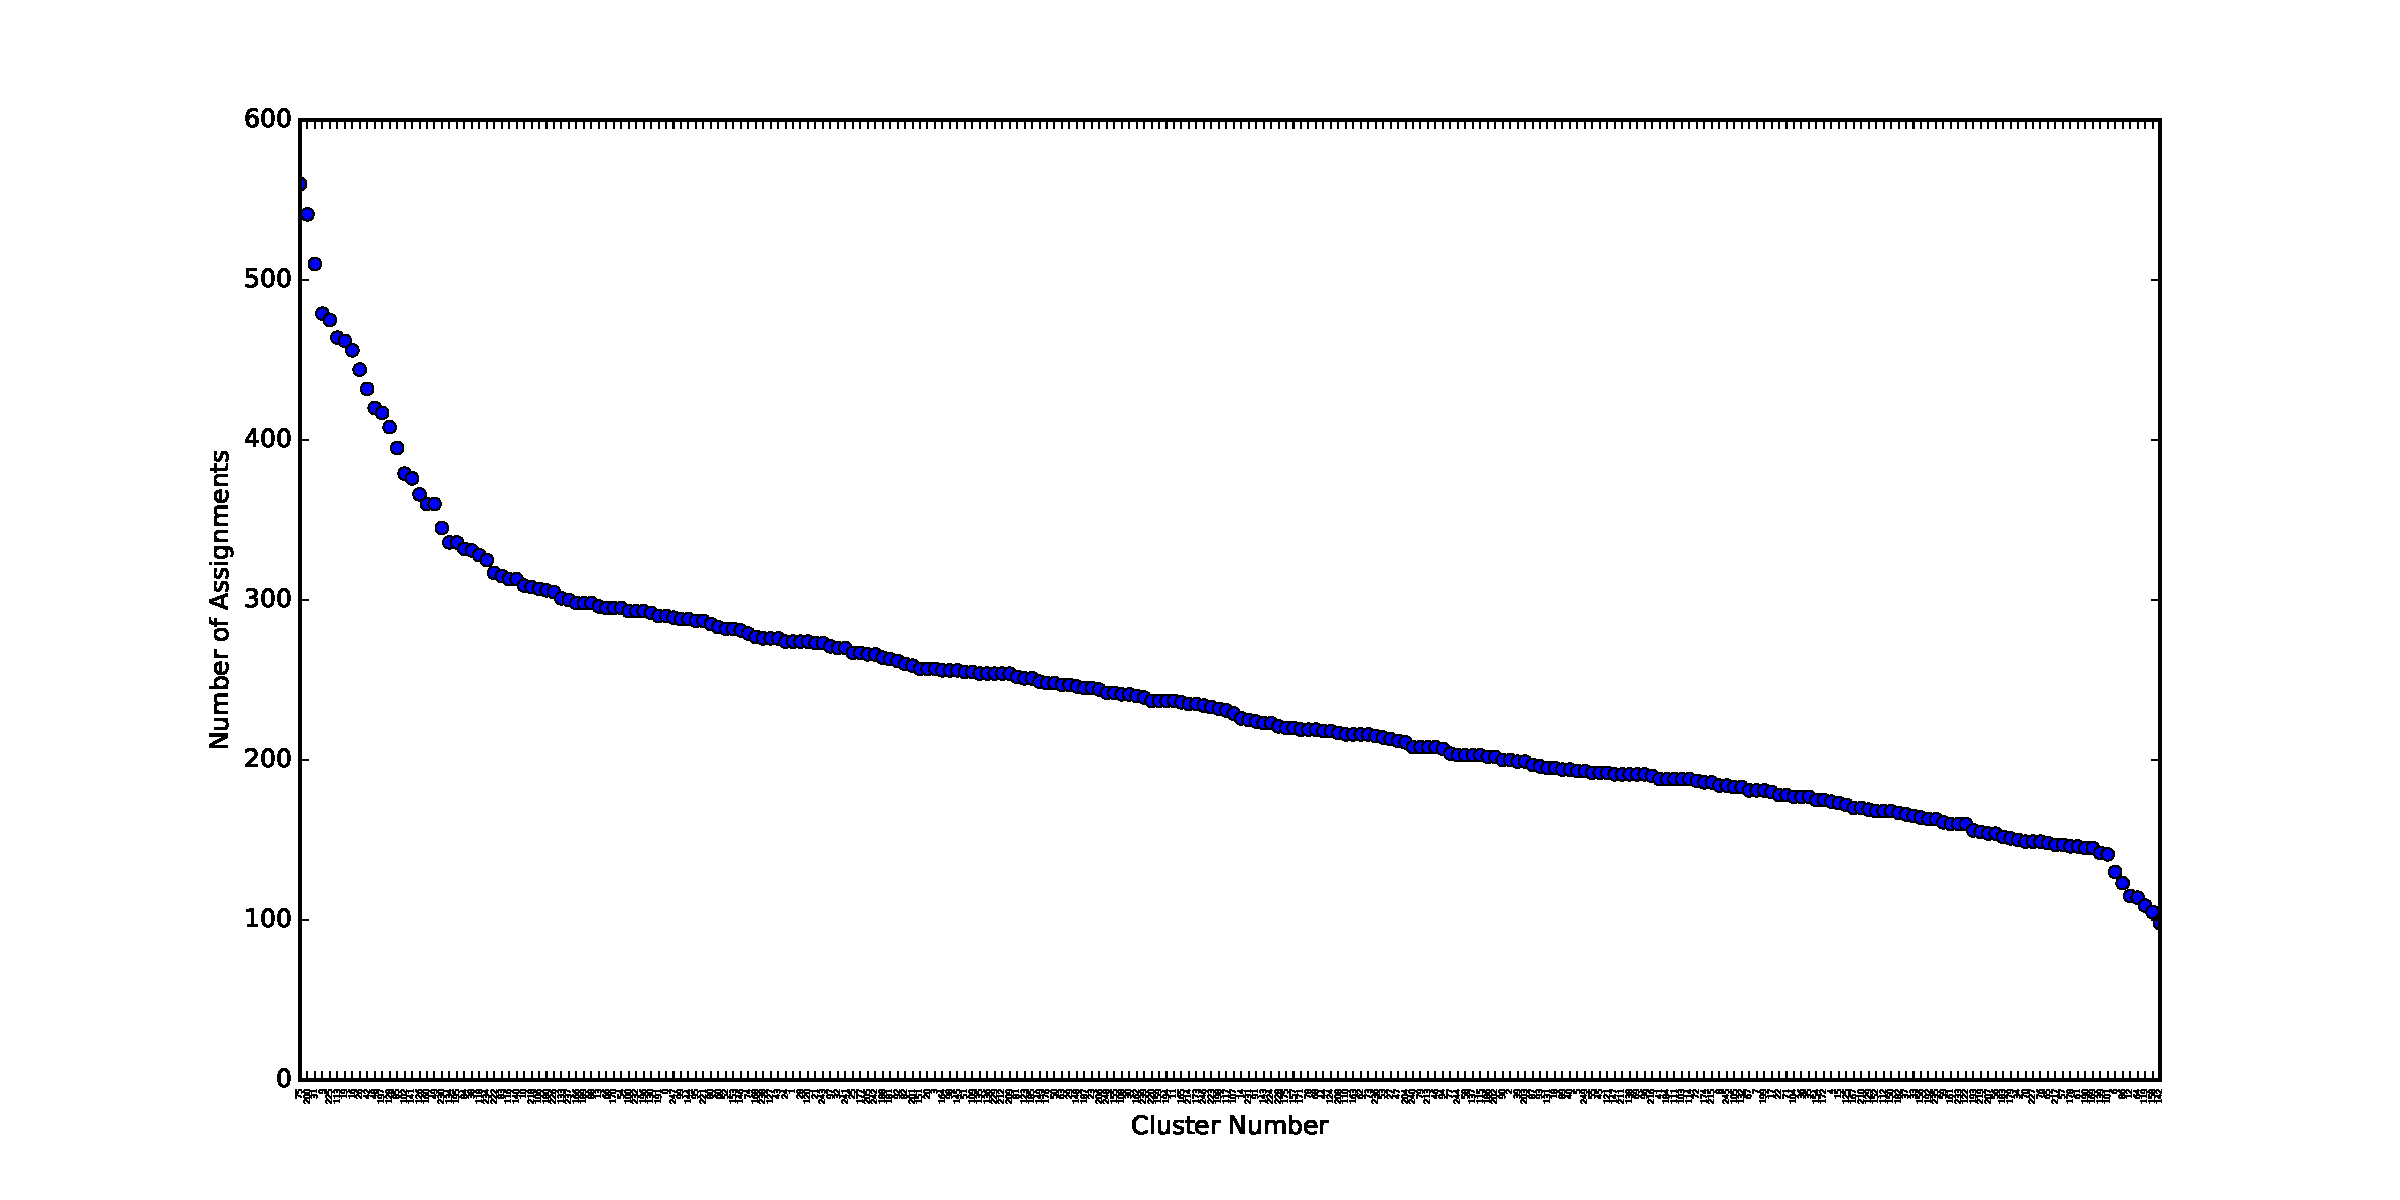
\includegraphics[width=\columnwidth]{k_250_num_assignments.pdf}
    \caption{Number of assignments per cluster for $k = 250$ clusters ordered in descending order.}
    \label{fig:k_250_num_assignments}
\end{figure}

Interestingly, there appears to be 3 regimes that each cluster center falls into.  The first regime involves the first 30 centers or so in which the number of assignments rapidly drops off, indicating that perhaps a smaller number of cluster centers really matter in terms of clustering, perhaps analogous to how PCA picks out the most important ``directions" in a dataset.  The next regime is a smooth, linear decrease in assignments due to clusters have less and less importance.  The final regime is a steep decrease in assignments and corresponds to the least important clusters.

\subsubsection*{5.1.2c}

In Fig.~\ref{fig:k_250_means}, I visualize the top 16 from my $k = 250$ centers my K-means algorithm learned on the MNIST training set in descending order for number of assignments.

\begin{figure}[H]
	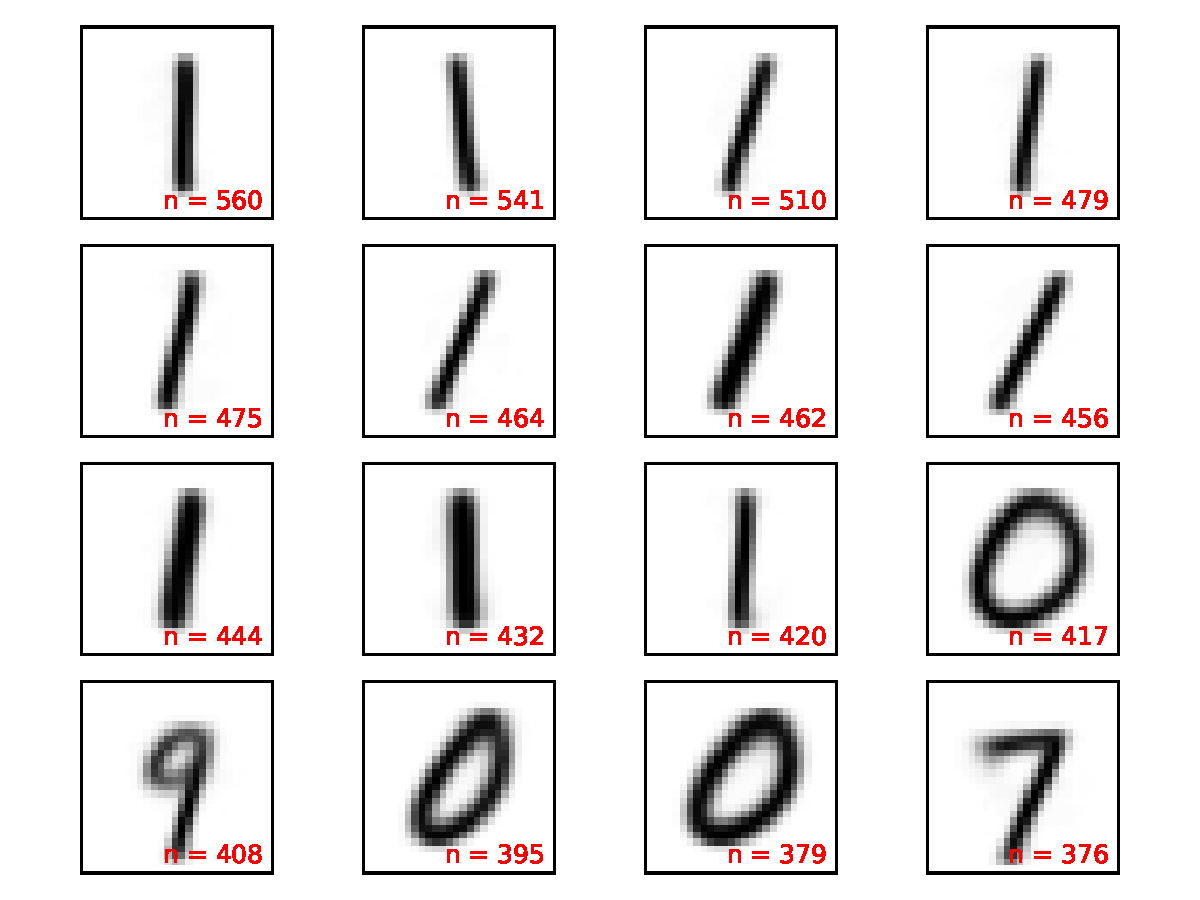
\includegraphics[width=\columnwidth]{k_250_means.pdf}
    \caption{Visualization of the $k = 250$ centers orders by number of members.  The number of members for each center is shown in each respective center's subplot in red in the lower-righthand corner.}
    \label{fig:k_250_means}
\end{figure}

From the figure it appears that the algorithm picked out various representations of a ``1'' as some of the most important cluster centers!  What I believe is going on is that a dominant feature in the MNIST digits is the right hand side of the digits.  Digits like 1, 3, 4, 5, 7, and 9 all have a more or less linear right hand side that, depending on who writes it, can slant in various orientations.  What this learning procedure did is identify, more or less, how certain digits tended to slope in some ways.  For example, one of the ``1''s is sloped in such a way that it looks like the base of a 7, so perhaps many 7s were attributed to that cluster.

\subsection*{5.2: Classification with K-means}

In this section I used my $k = 16$ and $k = 250$ K-means algorithms learned on the entire MNIST training set to classify digits.  I classified a digit by finding a label for each center based on the most frequent digit assigned to it.  For each sample, I found its closest center according to the squared Euclidean distance and used the label for that center.

\subsubsection*{5.2.1}

My $k = 16$ cluster K-means fit achieved 0/1 loss of 0.333 and 0.327 on the training and testing sets, respectfully.  Interestingly, the testing error was lower than the training error but I note that there was appreciable scatter between 0/1 losses for different fits using $k = 16$ on the training set.

\subsubsection*{5.2.2}

My $k = 250$ cluster K-means fit achieved 0/1 loss of 0.089 and 0.084 on the training and testing sets, respectfully.  Interestingly, the testing error was lower than the training error but I note that there was appreciable scatter between 0/1 losses for different fits using $k = 250$ on the training set.  The 0/1 loss in this case is roughly a factor of 3 lower than for the $k = 16$ case.  This likely occurred because the additional clusters can help distinguish between differently drawn digits of the same class, such as 4s written differently by different people.

\end{document}




















